\documentclass{beamer}

\usepackage{Vor2018glærur}

\title{Tölvunarfræði 2}
\subtitle{Vika 3}

\begin{document}

\begin{frame}
	\titlepage
\end{frame}

\section{Inngangur}

\begin{frame}{Leiðréttingar/útskýringar}
	\begin{itemize}
		\item Gildissvið breyta sem eru skilgreindar innan lykkju takmarkast við lykkjuna í C++
		\item \texttt{const} í C++ og \texttt{final} í Java hafa ekki nákvæmlega sömu merkingu
		\item Námundun við útskrift á \texttt{double} í straumi
		      \begin{itemize}
			      \item Sjá \texttt{precision.cpp}
		      \end{itemize}
	\end{itemize}
\end{frame}

\section{Fleiri hugtök úr hlutbundinni forritun}

\begin{frame}{Hugtök í hlutbundinni forritun}
	\begin{itemize}
		\item Þó nokkur hugtök eru notuð síendurtekið þegar hlutbundin forritun er rædd
		      \begin{itemize}
			      \item Erfðir \eng{inheritance} - hægt er að skilgreina klasa með vísun í annan klasa
			      \item Hjúpun \eng{encapsulation} og upplýsingahuld \eng{information hiding} - hægt er að vernda virkni hlutar með því að takmarka aðgang að innviðum hlutarins
			      \item Abstraction - hægt er að sýna upplýsingar til að vinna með hlut án þess að sýna hvernig hluturinn er útfærður
			      \item Polymorphism - mismunandi klasar geta brugðist við sama boði á mismunandi hátt (kemur oft í erfðum)
			      \item Fjölbinding \eng{overloading} - hægt er að skilgreina margar mismunandi merkingar fyrir sama fallsnafn eða virkja, aðgerð skilgreinist af samhengi
		      \end{itemize}
	\end{itemize}
\end{frame}

\begin{frame}{Erfðir}
	\begin{columns}
		\column{0.5\textwidth}
		\begin{itemize}
			\item Í hlutbundinni forritun eru klasar sem eiga margt sameiginlegt tengdir saman með erfðum
			\item Klasi B er skilgreindur með því að vísa í eiginleika klasa A
			      \begin{itemize}
				      \item Þá er talað um að B erfi frá (e. \emph{inherits from}) klasa A
			      \end{itemize}
			\item Getur verið gríðarlega gagnlegt til að forðast endurtekningar í kóða
		\end{itemize}
		\column{0.5\textwidth}
		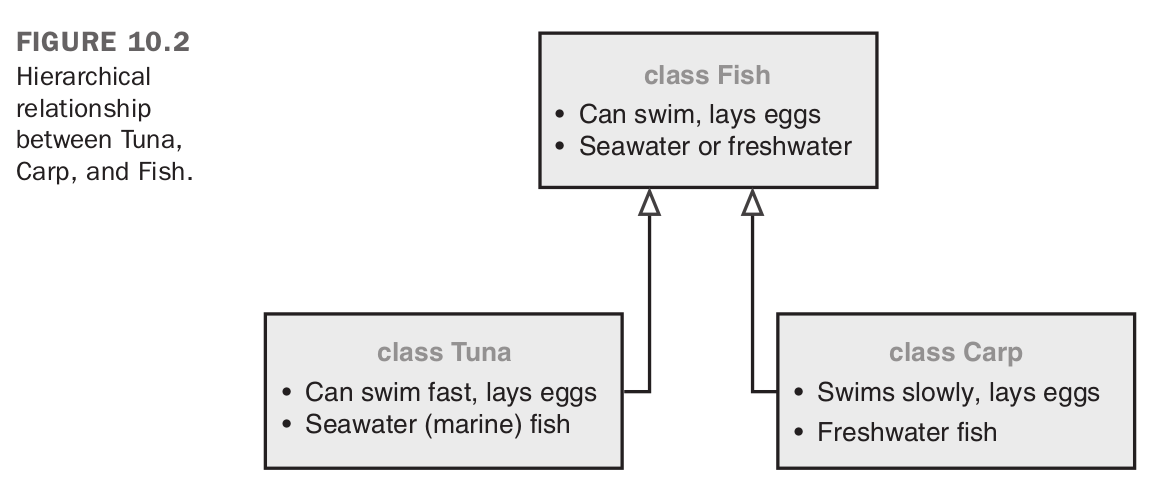
\includegraphics[width=\linewidth]{fishies}
	\end{columns}
\end{frame}

\begin{frame}[fragile]{Að skilgreina erfðir í C++}
	\begin{columns}
		\column{0.5\textwidth}
		\begin{itemize}
			\item Þegar klasi $B$ erfir frá $A$ fær $B$ aðgang að aðferðum og eiginleikum $A$
			\item Síðan höfum við val um hversu mikinn aðgang tilvik af $B$ hafa að eiginleikum $A$
			\item Venjulega munum við nota \texttt{public} aðgang
		\end{itemize}
		\column{0.5\textwidth}
		\begin{minted}[frame=lines, fontsize=\small]{cpp}
class A {
  // ... base class members
};
class B: access-specifier A {
  // ... derived class members
};
\end{minted}
	\end{columns}
\end{frame}

\begin{frame}[fragile]{Dæmi}
	Tvær gerðir af \texttt{Fish} sem eiga það sameiginlegt að geta framkvæmt \texttt{swim()}.
	\begin{columns}
		\column{0.45\textwidth}
		\cppfile[firstline=5, lastline=15, label=fishies.cpp, fontsize=\tiny, linenos=true]{Code/w3/fishies.cpp}
		\column{0.45\textwidth}
		\cppfile[firstline=17, lastline=20, label=fishies.cpp, fontsize=\tiny, linenos=true]{Code/w3/fishies.cpp}
		\cppfile[firstline=22, lastline=25, label=fishies.cpp, fontsize=\tiny, linenos=true]{Code/w3/fishies.cpp}
	\end{columns}
\end{frame}

\begin{frame}{Dæmi}
	\begin{itemize}
		\item Við getum látið tilvik af undirklösum vinna með aðferðir yfirklasa
		\item Getum ákveðið hvernig aðferðirnar eru bundnar
		      \begin{itemize}
			      \item Þegar forritið er þýtt (e. \emph{early binding})
			      \item Þegar forritið er keyrt og tag hlutarins ljóst (e. \emph{late binding})
		      \end{itemize}
		\item Getum tilgreint ``late binding'' með \texttt{virtual} lykilorðinu
		\item Skoðum \texttt{fishiesvirtual.cpp}
	\end{itemize}
\end{frame}

\begin{frame}{Fjölbinding}
	\begin{itemize}
		\item Við könnumst nú þegar við það að virki geti virkað á mismunandi hátt á mismunandi gögn!
		      \begin{itemize}
			      \item $1 + 2$ er ekki reiknað á sama hátt og $\frac{2}{3} + \frac{4}{3}$, þó við skiljum aðgerðina á sama hátt
			      \item Það sama á við í forritun - samlagning á tveimur \texttt{double} tölum fer ekki eins fram og samlagning á tveimur \texttt{int} tölum
		      \end{itemize}
		\item Í C++ getum við skilgreint hvaða merkingu virki á að hafa á tilvik klasanna okkar
	\end{itemize}
\end{frame}

\begin{frame}{Fjölbinding virkja í C++}
	Við getum skilgreint hvernig tvíundarvirkjar (með tvö viðföng) virka á tilvik af klasanum okkar með því að skilgreina nýja aðferð í klasanum:
	\begin{center}
		\texttt{return\_type operator\_type (parameter);}
	\end{center}
	Lítum á \texttt{lego.cpp} og \texttt{complex.cpp}
	\begin{center}
		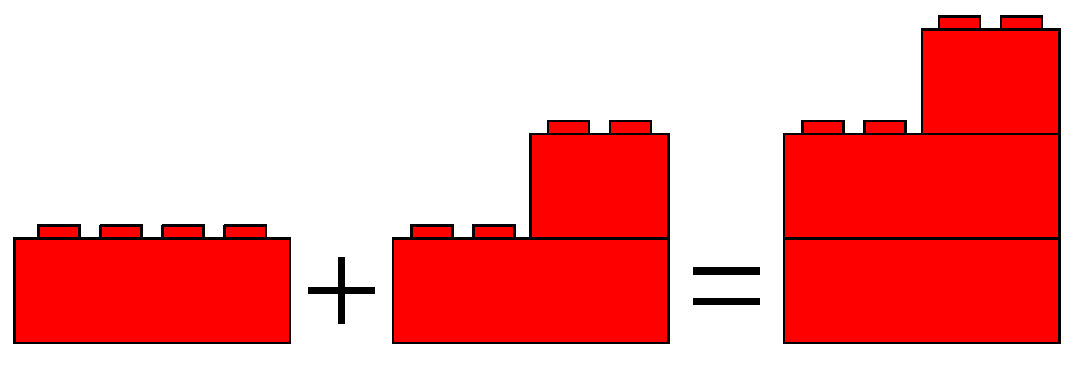
\includegraphics[width=0.7\textwidth]{lego-addition}
	\end{center}
\end{frame}

\section{STL og vector}

\begin{frame}{STL}
	\begin{itemize}
		\item STL stendur fyrir \emph{standard template library}
		\item Mikið safn klasa og forrita sem koma oft við sögu
		\item Inniheldur m.a.
		      \begin{itemize}
			      \item ``Geymslur'' \eng{containers}, útfærslur á þekktum gagnagrindum
			      \item Ítrara \eng{iterators} sem veita aðgang að gögnunum á staðlaðan hátt
			      \item Reiknirit \eng{algorithms} sem vinna á gögnunum í geymslunum, oft með því að nota ítrara
		      \end{itemize}
		\item Munum sjá margar gagnagerðir úr STL, skoðum fyrst \texttt{vector}
	\end{itemize}
\end{frame}

\begin{frame}{\texttt{vector}}
	\begin{itemize}
		\item Við höfum séð fylki í C-stíl
		\item Í mörgum algengum notkunartilvikum getur \texttt{vector} komið í stað fylkja
		\item Klasinn sér um minnisbókhald fyrir okkur
		      \begin{itemize}
			      \item Venjulega eru gögn \texttt{vector} tilviks geymd í kös þó að hluturinn sjálfur þurfi ekki að vera þar
			      \item Sér um eigin ruslasöfnun
		      \end{itemize}
		\item Hefur margar þægilegar hjálparaðferðir (\href{http://www.cplusplus.com/reference/vector/vector/}{yfirlit})
		\item Við gætum gert svipaðan klasa!
	\end{itemize}
\end{frame}

\begin{frame}{Bak við tjöldin}
	\begin{itemize}
		\item \texttt{vector} er ætlað að vera ``kvikt fylki'' sem getur höndlað mörg notkunartilvik, en bak við tjöldin þurfa samt að fara fram minnisúthlutanir
		\item Endurteknar minnisúthlutanir geta tekið mikinn tíma
		\item Lausnin sem \texttt{vector} fer - forúthlutun
		      \begin{itemize}
			      \item Skoðum \texttt{sizecapacity.cpp}
		      \end{itemize}
	\end{itemize}
\end{frame}

\subsection{STL hjálpartæki}

\begin{frame}{Ítrarar}
	\begin{itemize}
		\item Ítrarar (e. \emph{iterators}) eru að sumu leyti svipaðir bendum, notaðir til að vísa til sérstakra staka
		\item Dæmi:
		      \begin{itemize}
			      \item Föllin \texttt{begin()} og \texttt{end()} skila ítrurum sem vísa til fyrsta/síðasta staks
		      \end{itemize}
		\item Þykja nútímaleg leið til að vísa á stök
		      \begin{itemize}
			      \item Minni hætta á klaufavillum
			      \item Svipuð fyrirbrigði koma fyrir í mörgum nýrri forritunarmálum
		      \end{itemize}
		\item Meira um ítrara: \url{http://www.cplusplus.com/reference/iterator/}
	\end{itemize}
\end{frame}

\begin{frame}[fragile]{Ítrað yfir svið}
	Í stað þess að vísa sérstaklega í ákveðin stök eftir númeri er hægt að ítra yfir allt safnið \eng{iterate over range}.

	\cppfile[firstline=19, lastline=22, gobble=4, label=differentloops.cpp]{Code/w3/differentloops.cpp}

	Þessi gerð lykkju er kölluð ``range-based for loop'' í C++. Oft er talað um ``foreach'' lykkjur í öðrum málum.
\end{frame}

\begin{frame}{Reiknirit}
	\begin{itemize}
		\item Gagnagerðir í STL eru hannaðar til að virka með ýmsum hjálparföllum, m.a.
		      \begin{itemize}
			      \item \texttt{sort} - raðar safninu
			      \item \texttt{reverse} - snýr við röðun á safninu
			      \item \texttt{find} - finnur ákveðið stak í safninu
			      \item \texttt{transform} - beitir gefnu falli á safnið
		      \end{itemize}
		\item Til að nota föllin þarf \texttt{algorithm} hausinn
		\item Dæmi: \texttt{findexample.txt}
	\end{itemize}
\end{frame}

\section{Meira um þýðingu C++}

\subsection{Hausar og margar skrár}

\begin{frame}{Hausar og margar skrár}
	\begin{itemize}
		\item Við getum látið C++ forrit teygja sig yfir margar skrár
		\item Hægt að þýða margar í einu: \texttt{\$ g++ skra1.cpp skra2.cpp}
		      \begin{itemize}
			      \item Setjum skilgreiningar í \texttt{.h} skrár
			      \item Vísum í þær með \texttt{\#include}
			      \item GCC þekkir staðsetningar innbyggðra hausa eins og \texttt{iostream}
			      \item Þurfum ekki að þýða allar skrárnar ef sumar eru óbreyttar!
		      \end{itemize}
		\item Skoðum \texttt{myclass.cpp}, \texttt{myclass.h} og \texttt{runmyclass.cpp}
	\end{itemize}
\end{frame}

\subsection{Optimization levels}

\begin{frame}{Hverju skilar þýðandinn?}
	\begin{itemize}
		\item C++ þýðandi getur þýtt kóða á mismunandi hátt!
		\item Mikilvægt dæmi: Bestunarstillingar GCC
		      \begin{itemize}
			      \item Hægt er að ákveða hversu hart þýðandinn á að ganga fram við að búa til besta mögulega kóða
			      \item Sjálfgefið er að þýðingin sé hröð, ekki að hún skili hröðum kóða
			      \item \href{https://gcc.gnu.org/onlinedocs/gcc/Optimize-Options.html}{GCC Optimize Options}
		      \end{itemize}
		\item Sjá mismun: \href{http://godbolt.org/}{Godbolt}, \texttt{-S} valkostur GCC
	\end{itemize}
\end{frame}

\begin{frame}{Skilvirk endurkvæmni í GCC}
	\begin{columns}
		\column{0.3\textwidth}
		\begin{center}
			
\includegraphics[width=\linewidth]{stack-overflow}
		\end{center}
		\column{0.7\textwidth}
		\begin{itemize}
			\item Endurkvæm forrit geta falið í sér ansi mörg fallsköll
			      \begin{itemize}
				      \item Getur valdið vandamálum í C++ ef hlaðinn fær að vaxa
			      \end{itemize}
			\item GCC getur oft endurnýtt vakningafærsluna (e. \emph{stack frame} eða \emph{activation record}) ef við gefum þýðandanum rétta valkosti
			      \begin{itemize}
				      \item \texttt{-foptimize-sibling-calls} og fleiri
				      \item Innifalið í \texttt{-O2}, \texttt{-O3} og \texttt{-Os}
			      \end{itemize}
			\item Auðveldast er að endurnýta halaendurkvæm (e. \emph{tail recursive}) fallsköll
		\end{itemize}
	\end{columns}
\end{frame}

\begin{frame}{Halaendurkvæmni}
	\cppfile[firstline=4, lastline=10, fontsize=\scriptsize, label=recursivesum.cpp]{Code/w3/recursivesum.cpp}
	\cppfile[firstline=4, lastline=10, fontsize=\scriptsize, label=tailrecursivesum.cpp]{Code/w3/tailrecursivesum.cpp}
\end{frame}

\section{Lokaorð}

\begin{frame}{Takmörkun}
	\begin{itemize}
		\item Við kunnum ekki allt sem hægt er að læra í tengslum við C++ eftir þessar þrjár vikur
		\item En við eigum að kunna nóg til að\ldots
		      \begin{enumerate}
			      \item Forrita flest sem þarf í þessu námskeiði
			      \item Eiga auðvelt með að læra meira!
		      \end{enumerate}
	\end{itemize}
\end{frame}

\begin{frame}{Þessi glærupakki}
	Öll nafngreind forrit í þessum glærupakka, ásamt glærupakkanum sjálfum, má finna á  \href{https://github.com/Ernir/kennsluefni/tree/master/T2/Code/w3}{Github}.
\end{frame}

\begin{frame}{Næst}
	Hlutbundin forritun í Java, fjölnota klasar í Java (generics), skil (interfaces).
\end{frame}


\end{document}
